\section{Dimensioning Crowdsourcing Platforms}\label{sec:cloud:crowdsourcing}
\newcommand{\campaignIAT}{\ensuremath{A_C}\xspace}
\newcommand{\campaignSize}{\ensuremath{\Theta}\xspace}
\newcommand{\taskDuration}{\ensuremath{B}\xspace}
\newcommand{\meanTaskLength}{\ensuremath{E[B]}\xspace}
\newcommand{\numberOfWorkers}{\ensuremath{c}\xspace}
\newcommand{\workerUtilization}{\ensuremath{\rho}\xspace}
\newcommand{\campaignDuration}{\ensuremath{\delta}\xspace}
\newcommand{\preTaskProcessingDelay}{\ensuremath{E[D]}\xspace}
While the last sections dealt with dimensioning of resources in machine cloud systems, similar methodologies are applicable to crowdsourcing, or human-clouds.
Here, a crowdsourcing platform operator enables employers to distribute microtasks to workers.
In order to ensure the success of the platform, the operator has to ensure the satisfaction of both the employers, as they provide the main source of income, as well as the workers, the resource of the platform.
This tradeoff between employer satisfaction, i.e. time required before submitted tasks are completed, and worker satisfaction, i.e. income, has to be managed by the platform operator by carefully considering the number of workers employed at the platform.

To this end, in \refsec{sec:cloud:crowdsourcing:model} we first provide a mode for crowdsourcing platforms regarding the two identified metrics.
Then, we study parameters of a real world crowdsourcing platform in \refsec{sec:cloud:crowdsourcing:measurements}.
Finally, in \refsec{sec:cloud:crowdsourcing:performance_evaluation} we evaluate the provided model using the obtained parameters and discuss the tradeoff between employer and worker satisfaction from the point of view of the platform operator.

\subsection{Models of \headershortacr{GGSN} Implementations}\label{sec:cloud:virtualized_network_functions:model}

In this section we provide a model for a traditional \gls{GGSN} and discuss a model for a virtual \gls{GGSN} using \gls{NFV}.
In \gls{NFV} \cite{Nfv2013} static network middleboxes are replaced by commodity hardware.
The tasks solved by the original middleboxes are then solved by dedicated software.

\subsubsection*{Traditional GGSN}\label{sec:cloud:virtualized_network_functions:model:traditional_ggsn}
First, we give a model for a \emph{traditional} \gls{GGSN}, i.e. a static network component.
While we consider the \gls{GGSN} to be one fixed entity, it can in reality consist of multiple servers.
However, due to the fact that the \gls{GGSN} is purchased from a vendor as a middlebox, idle servers can be neither deactivated nor reused for other purposes.

\begin{figure}
  \centering
  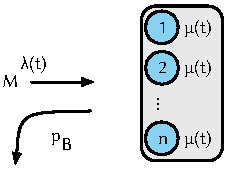
\includegraphics{cloud/virtualized_network_functions/model/figures/traditional_ggsn}
  \caption{Considered model of a traditional \headershortacr{GGSN}.}
  \label{sec:cloud:virtualized_network_functions:model:traditional_ggsn:model}
\end{figure}

We present an abstract queueing model for the traditional \gls{GGSN} in \reffig{sec:cloud:virtualized_network_functions:model:traditional_ggsn:model}.
New tunnels requests arrive according to a Poisson process with rate \(\lambda(t)\) at the \gls{GGSN}.
This server will support a maximum tunnel capacity of \(c\).
When this capacity is reached, blocking will occur and newly incoming tunnels requests are rejected.
Traditionally, \glspl{GGSN} can be expected to be overdimensioned in such a way that this rarely happens.
If the new tunnel is accepted, it will occupy one of the serving units of the server for the duration \(\mu(t)\) of the tunnel.
As stated earlier, we can not model the tunnel duration to be markovian, resulting in a  \(M/GI/c\) loss system.
In order to give quality of service guarantees the network operator is interested in the system's blocking probability \(\blockingprobability\), which we consider to be a key metric of our model.
Additionally, the previously described diurnal patterns can also be modelled by adjusting the arrival and serving process distributions for each time of day.
This alternatively also allows just to investigate the busy hour and thus the system's peak load.

\subsubsection*{\headershortacr{GGSN} using Network Function Virtualisation}\label{sec:cloud:virtualized_network_functions:model:virtual_ggsn}
Next, we introduce concepts from \gls{NFV}, i.e. the idea to replace middleboxes with commodity hardware as an extended model in \reffig{sec:cloud:virtualized_network_functions:model:virtual_ggsn:model}.
This allows us to realise benefits from cloud computing, as we are now able to scale out, instead of up.
The assumptions of the Markov arrival process \(\lambda(t)\) and the serving time distributions \(\mu(t)\) are carried over.
However, instead of one server processing every tunnel, this model assumes that there are up to \(s_{max}\) virtualised servers \(s_i\).
Each of these is less powerful than the traditional \gls{GGSN}, having a tunnel serving capacity of \(c_i \ll c\) and a total system capacity of \(c_{max} = s_{max} \times i\).

\begin{figure}
  \centering
  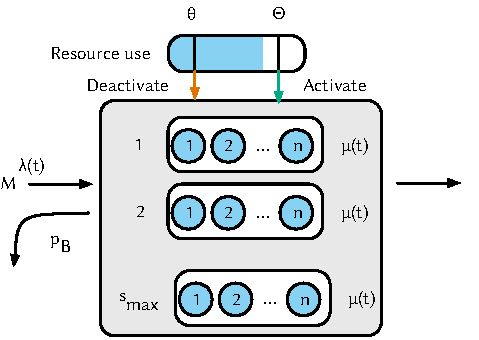
\includegraphics{cloud/virtualized_network_functions/model/figures/virtual_ggsn}
  \caption{Considered model of a virtualised \headershortacr{GGSN}.}
  \label{sec:cloud:virtualized_network_functions:model:virtual_ggsn:model}
\end{figure}

In its initial state, for efficiency, all but a small portion of the server instances are considered to be disabled.
Only, when a certain condition is reached, a new server instance is provisioned.
As a simple example, one instance could be kept in reserve for upcoming requests and an additional would be provisioned as soon as the reserve is used.
Similar rules should apply to the shut-down of servers and form a hysteresis with the boot condition.
For example it would be possible to keep at least one server in reserve but never more than two.

If these conditions are not carefully selected and are in tune with the expected boot time of an instance, additional blocking can occur.
Despite not having reached its maximum capacity, this system would still reject tunnel requests during the provisioning phase when no tunnel slots are available.
This could be remedied by a request queue.
However, this would introduce additional complexity to the system without providing real benefit, as mobile devices or applications will repeat their attempts and would timeout when the request is taking too long.

To place incoming tunnel state on one of the available servers a load balancer is required.
To ensure that the system in run time can scale down to its actual needs, the balancer should place tunnels on servers that are the fullest, keeping the reserve free.
It may even migrate tunnel state from almost empty servers away so that these can be shut down, when the shut-down condition is fulfilled.
Keeping instance close to their capacity should also have no impact on the performance a mobile device associated to a specific tunnel experiences.

\section{Measurements and Models of Content Delivery Networks}\label{sec:aslevel:measurements}

The most popular P2P overlay network today is BitTorrent.
BitTorrent is still responsible for a large portion of Internet traffic \cite{cisco2016,wamser2010}.
% In particular, BitTorrent networks generate a lot of inter-ISP traffic, which is often costly for the ISPs. One approach to optimize the traffic flows, which received a lot of attention is Application Layer Traffic Optimization (ALTO), to increase the efficiency of BitTorrent and to reduce the amount of inter-ISP traffic and costs. Evaluations of such approaches have been conducted mostly in controlled, artificial scenarios. Examples for such scenarios are simulations with homogeneous peer distributions across ISPs, the evaluation of simple topologies, like the star topology with a tier--1 ISP in the center. However, in today's Internet the inter-ISP traffic routing is based on a complex topology defined by inter-ISP relationships, e.g., peering or transit, and ISP classifications such as \tier, large and small ISPs, and stub ISPs. Hence, these economic relations play an important role in the actual Internet traffic flow. However, this topology of the Internet is not taken into account by most evaluations of P2P guidance approaches, which limits the practical relevance of the results.
%Furthermore, it is an open question how much BitTorrent traffic is located in which region of the Internet.
%This is a prerequisite in order to estimate the potential of ALTO mechanisms.
In \refsec{aslevel:measurements:bittorrent} we give an overview on measurement studies of live BitTorrent networks and show different approaches to reduce costly traffic discussed in the ALTO working group of the IETF.

We summarize related work in the field of distributed active measurements of CDNs and give a short introduction in the principles of crowdsourcing in \refsec{aslevel:measurements:cdn}.

\subsection{Measurements and Models of BitTorrent Networks}\label{aslevel:measurements:bittorrent}

The measurements and models for the distribution of peers on ASs indicate the distribution of hosts on the Internet and help to identify groups that are interested in the same content.
This information can be used for traffic models and to optimize CDNs on AS level. 
As basis of our methodology for modeling inter-ISP BitTorrent traffic in \refsec{sec:aslevel:p2p}, the results in \cite{Hossfeld2011} are revisited. The authors provide measurements of a large number of live BitTorrent swarms taken from popular index servers such as \emph{The Pirate Bay}, \emph{Mininova}, and \emph{Demonoid}. Using the IP addresses of the peers, the authors associate every peer with its AS and estimate the potential of ALTO mechanisms based on the differentiation between local peers (peers in the same AS) and remote peers located in other ASs. In contrast, we consider the actual Internet topology in this work, i.e., the inter-ISP relations, the ISP classification in the Internet hierarchy, and the AS paths between the peers in order to estimate the optimization potential of ALTO mechanisms.

The authors of \cite{Kryczka2011} use the peer exchange protocol (PEX) in order to measure the neighbor set of all peers participating in a number of live BitTorrent swarms. Based on this information, they model the graph topology of the swarms and compare the structure to random graphs. They also investigate clustering of peers within ASs and countries, but do not focus on inter-AS relations and AS paths between peers as we do in this chapter.

In addition, there are measurement studies that examine and model distinct features of BitTorrent networks. In \cite{Izal2004}, a single swarm was measured for five months with a focus on the download times of the peers. Additional parameters such as the peer inter-arrival times in the swarm, their upload capacity and their online time are considered in \cite{Pouwelse2005}. The authors of \cite{Guo2005} investigate these parameters also in multi-swarm scenarios. Finally, \cite{Zhang2010} measures \unit[4.6]{million} torrents to provide an overview of the entire BitTorrent ecosystem with its different communities and index servers.
While the distribution of peers in the Internet is also studied in this chapter, none of these works focuses on the location of the peers in the Internet and the AS paths between the peers, which is a major aspect of this chapter.

% \subsection{ALTO Mechanisms and Their Performance Evaluation}
%
Various mechanisms to reduce the inter-ISP traffic generated by BitTorrent and other P2P applications are currently being investigated. Besides caching of BitTorrent traffic \cite{Lehrieder2010a,Lehrieder2012,Pacifici2012}, which might involve legal issues, changing standard BitTorrent algorithms is a promising approach. The authors of \cite{Aggarwal2007} propose to use an oracle service provided by the ISP guiding the peers in their peer selection process. The evaluation uses a Gnutella network and shows that intra-AS traffic is increased significantly without a negative impact on the overlay graph. Similar approaches are proposed for BitTorrent. Bindal et al. \cite{Bindal2006} reduce the inter-ISP traffic by modifying the neighbor set of the BitTorrent peers, which can be done at the tracker or enforced by the ISPs using deep packet inspection. Their simulations use a uniform peer distribution over ASs and show a high optimization potential of this approach. The authors of \cite{Xie2008} propose to use \emph{iTrackers} to guide the peers and formulates an optimization problem to find the best neighbor sets. Finally, Oechsner et al. \cite{Oechsner2009} propose to change the choke algorithm of BitTorrent to further reduce inter-ISP traffic and evaluate it via simulations in homogeneous scenarios. The BitTorrent plugin \emph{Ono} \cite{Choffnes2008} uses the servers of CDNs as landmarks and estimates the proximity of two peers by the similarity of the CDN re-direction behavior.
%

The authors of \cite{gkantsidis2006planet} investigate analytically the capabilities of a P2P-based content distribution network and the impact of locality. In contrast to our work, they use traffic characteristics which arise from software updates and do not consider AS relationships.
A set of evaluations of ALTO mechanisms uses scenarios inspired by measurements of live BitTorrent swarms \cite{Cuevas2011,Blond2011,Lehrieder2011}. The studied scenarios consider heterogeneous peer distributions where some ASs contain more peers of a specific swarm than others. Nevertheless, they do not take into account inter-AS relations and the AS paths between two peers. This is different in our study. Using the AS affiliation of peers and the data obtained from Caida.org, we infer the actual paths of the BitTorrent connections in the Internet. In addition, we focus on the inter-ISP relations and investigate to which degree selfish ISPs profit from recommending their peers to preferentially use connections to peers located in lower tier ASs.

\subsection{Measurements of Content Delivery Networks}\label{aslevel:measurements:cdn}
There already exist a number of publications which study the structure of CDNs.
Much focus is put on the YouTube CDN and its selection of video servers, as it is the most popular CDN for video content.
A distributed active measurement platform is necessary for these evaluations, because the CDN mechanisms consider the client locations, both geographical as well as in terms of the connected access network.
Recently, the physical server distribution of NetFlix's CDN was mapped in \cite{bottger2016open}, using a DNS crawler and exploiting the naming scheme of the cache servers.
%It is differed between ISP and IXP deployment of the servers and find that a region-specific deployment of the servers is required dependent on the different markets.
%Deploying within ISPs takes time, so IXP deployment reflects the phase in the ongoing process of deploying within ISPs.
In \cite{torres2011dissecting}, two university campus networks and three ISP networks were used to investigate the YouTube CDN from vantage points in three different countries.
%The results show that locality in terms of latency is not the only factor for video server selection.

While the view of five different ISPs on a global CDN is still narrow, the authors of \cite{adhikari2011you} used PlanetLab to investigate the YouTube server selection strategies and load-balancing.
They find that YouTube massively deploys caches in many different locations worldwide, placing them at the edge of the Google autonomous system or even at ISP networks.
The work is enhanced in \cite{adhikari2012vivisecting}, where they uncover a detailed architecture of the YouTube CDN, showing a 3-tier physical video server hierarchy.
Furthermore, they identify a layered logical structure in the video server namespace, allowing YouTube to leverage the existing DNS system and the HTTP protocol.

However, to assess the expansion of the whole YouTube CDN and its cache locations in access networks, the PlanetLab platform, which is located solely in NRENs, is not suitable, since it does not reflect the perspective of end users in ISP access networks.
Therefore, a different distributed measurement platform is used in \cite{rafetseder2011exploring} which runs on end user equipment and thus implies a higher diversity of nodes and reflects the perspective of end user in access networks.
However, the number of nodes that was available for the measurement is too small to obtain a global coverage of vantage points

To achieve both, the view of access networks and a high global coverage with a large number of measurement points, the participation of a large number of end users in the measurement is necessary.
Bischof et al. \cite{bischof2011crowdsourcing} implemented an approach to gather data from P2P networks to globally characterize the service quality of ISPs using volunteers.

In contrast to this we propose using a commercial crowdsourcing platform to recruit users running a specially designed measurement software, and therewith, act as measurement probes.
Crowdsourcing is an emerging service in the Internet that enables outsourcing jobs to a large, anonymous crowd of users~\cite{articles2013-113}.
So called \emph{Crowdsourcing platforms} act as mediator between the users submitting the tasks, the \emph{employers}, and the users willing to complete these tasks, the \emph{workers}.
All interactions between workers and employers are usually managed through these platforms and no direct communication exists, resulting in a very loose worker-employer relationship.
The complexity of crowdsourcing tasks varies between simple transcriptions of single words~\cite{vonAhn2008} and even research and development tasks~\cite{innocentive}.
Usually, the task descriptions are much more fine granular than in comparable forms in traditional work organizations~\cite{conf2011-417}.
This small task granularity holds in particular for \emph{micro-tasks}, which can be completed within a few seconds to a few minutes.
These tasks are usually highly repetitive, e.g., adding textual descriptions to pictures, and are grouped in larger units, so called \emph{campaigns}.
In comparison to other approaches using volunteers, this approach offers better scalability and controllability, because the number and origin of the participants can be adjusted using the recruiting mechanism of the crowdsourcing platform.
% This is confirmed by Table~\ref{tab:CvsS} which compares a crowdsourcing study with a social network study quantitatively. The crowdsourcing study  is described in \cite{bookchapter2013-18}. The study is designed to assess the subjective QoE for multimedia applications, like video streaming.
% The same study was conducted additionally in a social network environment for recruiting test users.
% Table~\ref{tab:CvsS} shows that acquiring people in crowdsourcing platforms takes very short time compared to asking volunteers in a social network, which allows adding participants easily.
% Furthermore, the completion time of the campaign of 31 hours is much shorter compared to the 26 days for the social network campaign.
% Finally, in the crowdsourcing campaign workers can be selected according to their country, which allows distributing the campaign on many different countries. In the social network the coverage of countries depends on the network of user groups, which spread the campaign.
% Hence, it is easy to control the number and origin of subjects participating in a crowdsourcing campaign and the completion time is considerably fast, which makes the campaign scalable and controllable. The price you pay is the reward for the workers that summed up to a total of 16 Euro for that campaign.
%
% \begin{table}[tb]
% \caption{Quantitative Comparison: Crowdsourcing / Social Network Study.} \label{tab:CvsS}
% \begin{center}
% {\footnotesize
% 	\begin{tabular}{|p{.29\textwidth}|p{.29\textwidth}|p{.29\textwidth}|} \hline
% 		\textbf{} & \textbf{Crowdsourcing (C)} & \textbf{Social network (S)} \\ \hline
% 		\textbf{Implementation time} & about 2 weeks; test implemented via dynamic web pages, application monitoring & same as for (C) \\ \hline
% 		\textbf{Time for acquiring people} & 5 minutes & 2 hours, as users (groups) were asked individually \\ \hline
% 		\textbf{Campaign submission cost} & 16 Euro & 0 Euro \\ \hline
% 		\textbf{Subject’s reward} & 0.15 Euro & 0 Euro \\ \hline
% 		\textbf{Number of test conditions} & 3 & 3 \\ \hline
% 		\textbf{Advertised  people} & 100 & 350 \\ \hline
% 		\textbf{Campaign completion time} & 31 hours & 26 days; strongly depends on advertised user groups however \\ \hline
% 		\textbf{Participating users} & 100 & 95 \\ \hline
% 		\textbf{Reliable users (very strict filtering of users)} & 30 & 58 \\ \hline
% 		\textbf{Number of different countries of subjects} & 30 & 3; strongly depends on users groups however \\ \hline
% 		\end{tabular}
% }
% \end{center}
% \end{table}


%To the best of our knowledge, this is the first work which evaluates a gl
%To the best of our knowledge this is the first work which uses crowdsourcing for a distributed active measurement platform.

\subsection{Evaluation of Platform Characteristics on Considered Metrics}\label{sec:cloud:crowdsourcing:performance_evaluation}

In this section we use the simulative model introduced in \refsec{sec:cloud:crowdsourcing:model} and the measurements obtained from the Microworkers platform in order to analyse the impact of different parameters on the considered metrics.
First, we study the impact of campaign inter-arrival times.
Then, we study tradeoffs between metrics of interest for the different stakeholders.
The results presented in this section can be used as guidelines for platform operators, in order to ensure that both stakeholders are sufficiently satisfied.

\subsubsection*{Impact of Campaign Inter-arrival Distributions}

Campaign inter-arrival times \campaignIAT influence both the work load of the individual workers \workerUtilization as well as the mean time required before a worker starts working on a task \preTaskProcessingDelay.
From the perspective of an operator, understanding the influence of different inter-arrival processes is important.
As shown in \refsec{sec:cloud:crowdsourcing:measurements}, the gamma distribution can be used to approximate the campaign inter-arrival times \campaignIAT as seen on the crowdsourcing platform Microworkers.
In this section, we study the impact of such different processes by utilising the parameter space afforded by the gamma distribution and considering the impact on the metrics utilisation \workerUtilization and mean task pre-processing delay \preTaskProcessingDelay.

The characteristics of the gamma distribution change depending on the parameters shape \(\alpha\) and rate \(\beta\).
While both shape and rate influence the mean
\begin{equation*}
E[\campaignIAT] =  \frac{\alpha}{\beta}
\end{equation*}
and variance
\begin{equation*}
\Var[\campaignIAT] =  \frac{\alpha}{\beta^2}
\end{equation*}
of the campaign inter-arrival times \campaignIAT, only the shape influences the skewness
\begin{equation*}
\Skew[\campaignIAT] =  \frac{2}{\sqrt{\alpha}}
\end{equation*}
of the distribution.

For a shape of \(\alpha = 1\) the gamma distribution given by as
\[
P(A_c=t) \sim \frac{\beta^\alpha}{\Gamma(\alpha)} x^{\alpha-1} e^{-{\beta}t}
\]
degenerates to an exponential distribution with a \gls{PDF} given as
 \[
a_c(t) = \beta e^{\beta t}
 \]
due to definition of the gamma function as \(\Gamma(1) := 1\).

Increasing of the shape for the same rate changes the form of the distribution from an exponential type to a distribution which is similar to a normal distribution.
By increasing the rate for the same shape the tightness of the distribution is modified.
For rate parameters \(\alpha < 1\) this results in a distribution with a long tail.
The increase of the rate decreases the breadth of the distribution.
Transferred to the campaign inter-arrival process \campaignIAT different shape and rate settings can be used to model different task types and varying the business of the platform.
The range of the inter-arrival times is given by the rate and the shape defines the weighing of the different times.
A lower shape means more campaigns arrive in bursts in combination with longer time periods without any campaign arrival.

Next, we use our simulation model introduced in \refsec{sec:cloud:crowdsourcing:model} with the campaign size distribution \campaignSize and task completion times \taskDuration obtained in \refsec{sec:cloud:crowdsourcing:measurements} for different campaign inter-arrival times to study the impact on the utilisation.
Only stable systems, i.e., crowdsourcing platforms with a utilisation \(\workerUtilization < 1\) are considered in the following.

\begin{figure*}
	\centering
	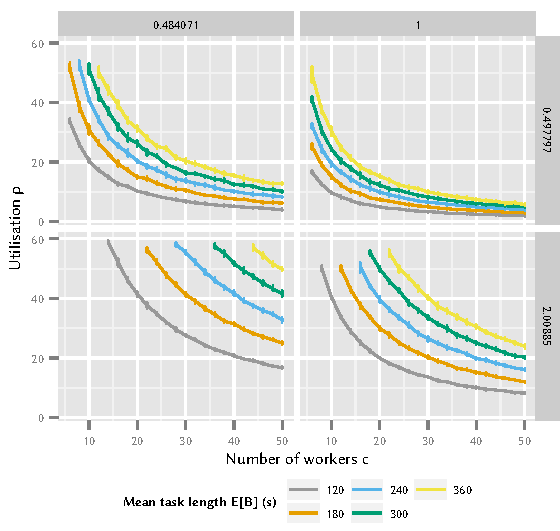
\includegraphics{cloud/crowdsourcing/numerical_evaluation/figures/parameter_utilization}
	\caption{Utilisation \workerUtilization for different campaign inter-arrival times \campaignIAT.}
	\label{fig:cloud:crowdsourcing:performance_evaluation:distributions:parameter_utilization}
\end{figure*}

Independent of the campaign inter-arrival time distribution \campaignIAT and the number of workers \numberOfWorkers, we see in \reffig{fig:cloud:crowdsourcing:performance_evaluation:distributions:parameter_utilization} that the introduction of more complex tasks in the platform by means of a higher mean task length \meanTaskLength increases the utilisation \workerUtilization.
The same number of workers \numberOfWorkers now require more time to process the same number of tasks.
Furthermore, for the same campaign inter-arrival times \campaignIAT and mean task lengths \meanTaskLength, increasing the number of workers \numberOfWorkers decreases the utilisation \workerUtilization, as a higher number of workers has to compete for the same number of tasks.
For different shapes \(\alpha\) of the campaign inter-arrival times \campaignIAT and the same rate \(\beta\), with all other parameters fixed, we observe a decrease of the shape results in an increase in utilisation \workerUtilization.
A decrease of the shape \(\alpha\) directly decreases the mean campaign inter-arrival time \(E[\campaignIAT]=\frac{\alpha}{\beta}\) and increases the rate \(\frac{1}{E[\campaignIAT]}\) of incoming campaigns, which increases the utilisation \workerUtilization.
The same argument can be applied to the rate parameter of the campaign inter-arrival time distribution \campaignIAT.
An increase of the rate \(\beta\) again influences the mean \(E[\campaignIAT]\) and the rate of the campaign inter-arrival time \campaignIAT resulting in an increased utilisation \workerUtilization.

\begin{figure*}
	\centering
	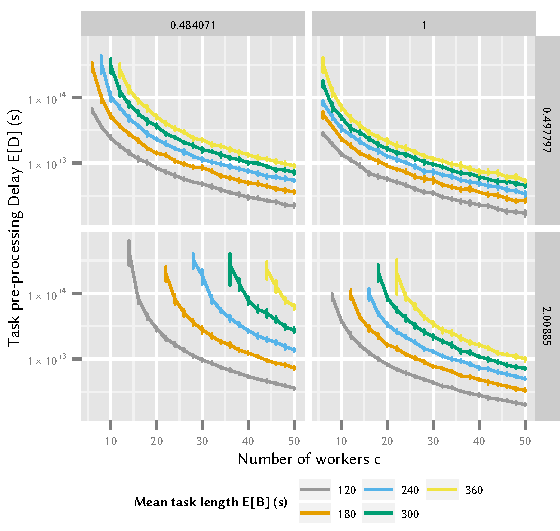
\includegraphics{cloud/crowdsourcing/numerical_evaluation/figures/parameter_task_delay}
	\caption{Mean task pre-processing delay \preTaskProcessingDelay for different campaign inter-arrival times \campaignIAT.}
	\label{fig:cloud:crowdsourcing:performance_evaluation:distributions:parameter_task_delay}
\end{figure*}

In \reffig{fig:cloud:crowdsourcing:performance_evaluation:distributions:parameter_task_delay} we consider the impact of different campaign inter-arrival time characteristics \campaignIAT on the task pre-processing delay \(\preTaskProcessingDelay\).
For a fixed number of workers \numberOfWorkers and campaign inter-arrival distribution \campaignIAT a larger mean task duration \taskDuration also increases the mean task pre-processing delay \preTaskProcessingDelay.
As more tasks have to enter the queue, tasks which would not have been queued for lower task length now suffer queueing delay.
For a fixed task length \taskDuration and campaign inter-arrival distribution \campaignIAT, we see that increasing the number of workers \numberOfWorkers results in a decreased task pre-processing delay \preTaskProcessingDelay.
The waiting probability decreases due to the higher capacity of the platform, resulting in a lower waiting time per task.
Next, we consider the shape of the campaign inter-arrival time for fixed other parameters.
The curves show that increasing the shape decreases the mean task pre-processing delay \preTaskProcessingDelay.
This is caused by an increasing mean \(E[\campaignIAT]\) of the inter-arrival times which results in a decrease of the campaign arrival rate.
Thus, the platform contains fewer tasks for the same number of workers \numberOfWorkers and fewer tasks have to wait for completion.
The effect is more obvious for higher traffic intensities.

Finally, we consider the effect of an increased rate \(\beta\) while keeping all other parameters fixed.
An increased campaign inter-arrival rate increases the task pre-processing time \preTaskProcessingDelay, as the number of campaigns arriving at the platform is increased.
The increase of the rate \(\beta\) decreases the variance of the campaign inter-arrival times distribution.
For greater values of \(\beta\), the mean campaign inter-arrival time \(E[\campaignIAT]\) decreases as the campaign inter-arrival rate increases.
Thus, more tasks arriving at the platform and have to be completed with the same number of workers \numberOfWorkers.

Based on these observations, we conclude that while both shape and rate influence the metrics utilisation \workerUtilization and mean task pre-processing delay  \preTaskProcessingDelay, the rate parameter \(\beta\) of the gamma distribution has a higher influence on the considered metrics.
In order to account for the higher influence of the rate on the considered metrics, we fix the shape parameter \(\alpha\) of the gamma distribution to the value \(0.484071\) obtained in \refsec{sec:cloud:crowdsourcing:measurements} for the next section and focus on different rate parameters \(\beta\).

\subsubsection*{Tradeoff Considerations for Platform Operators}

A crowdsourcing platform operator's business success depends on the satisfaction of the main stakeholders, i.e., the employers and workers.
As discussed in \refsec{sec:cloud:crowdsourcing:model}, workers are interested in a high utilisation \(\workerUtilization\), due to the fact that this correlates with their payment.
Employers are interested in having their tasks completed as fast as possible, i.e., in an as small as possible task pre-processing delays \(\preTaskProcessingDelay\).
The interests of the stakeholders are opposing as lower task pre-processing delays \(\preTaskProcessingDelay\) can be achieved by hiring more workers, which in turn results in a lower utilisation \(\workerUtilization\).
Thus, the platform operator is forced to consider a tradeoff between worker and employer satisfaction, which we consider in this section.
The impact of different campaign inter-arrival rates \campaignIAT on worker and employer satisfaction for the specific platform can be evaluated by following the coloured lines in \reffig{fig:cloud:crowdsourcing:performance_evaluation:tradeoff:pareto}.

\begin{figure*}
	\centering
	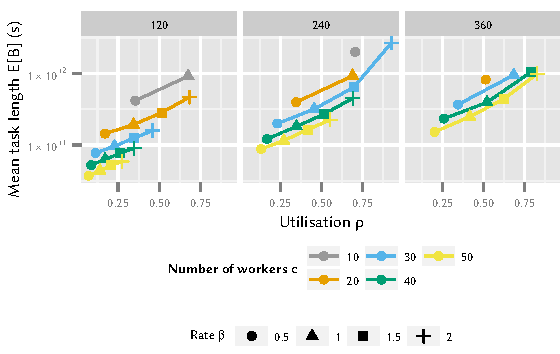
\includegraphics{cloud/crowdsourcing/numerical_evaluation/figures/pareto}
	\caption{Tradeoff analysis between utilisation \workerUtilization and mean task pre-processing delay \preTaskProcessingDelay.}
	\label{fig:cloud:crowdsourcing:performance_evaluation:tradeoff:pareto}
\end{figure*}

Given a fixed number of workers \numberOfWorkers, decreases in the campaign inter-arrival rate \(\beta\) result in lower utilisation \workerUtilization and longer mean task pre-processing delays \preTaskProcessingDelay.
The effects on the utilisation \workerUtilization and the mean task pre-processing time \preTaskProcessingDelay decrease for a larger amount of workers \numberOfWorkers.
This means a platform with a larger number of workers is more robust against fluctuations in the rate of incoming campaigns \(\beta\) than a system with a small number of workers \numberOfWorkers.

Independent of the considered task duration \taskDuration, we observe that increasing the number of workers \numberOfWorkers, e.g. advertising the platform, decreases both the mean task pre-processing delay \preTaskProcessingDelay as well as the utilisation \workerUtilization.
However, this decrease is not linear.
This means that a small increase of the number of workers \numberOfWorkers reduces the utilisation \workerUtilization, which is generally not desired.
However, this small degradation of the utilisation \workerUtilization results in an over-proportional reduction of the mean task pre-processing delay \preTaskProcessingDelay.
Thus, it is advisable to slightly overdimension the number of workers \numberOfWorkers to optimise the tradeoff between utilisation \workerUtilization and mean task pre-processing delay \preTaskProcessingDelay.
